% Progress report: PEFT for foundation models in federated learning -- text-based person search.
% Build:  cd paper && python3 scripts/gen_tables.py && latexmk -pdf -outdir=build main.tex
% Overleaf: compiler = pdfLaTeX (default). Do not run a single pdflatex pass: it gives "??".
% Writing style: ASD-STE100 (Simplified Technical English).
\documentclass[11pt,a4paper]{article}

\usepackage[T1]{fontenc}
\usepackage[utf8]{inputenc}
\usepackage{mathptmx}
\usepackage[scaled=0.92]{helvet}
\usepackage{courier}
\usepackage{amsmath,amssymb}
\usepackage[a4paper,margin=2.5cm]{geometry}
\usepackage{microtype}
\usepackage{booktabs,array,tabularx}
\usepackage{xcolor}
\usepackage{graphicx}
\usepackage{enumitem}
\setlist{itemsep=1pt,topsep=3pt}
\usepackage{caption}
\captionsetup{font=small,labelfont=bf}
\usepackage[ruled,vlined,linesnumbered]{algorithm2e}
\usepackage{tikz}
\usetikzlibrary{positioning,arrows.meta,calc}
\usepackage{pgfplots}
\usepgfplotslibrary{groupplots}
\pgfplotsset{compat=1.17}
\usepackage{float}
\usepackage[export]{adjustbox}
\usepackage{tcolorbox}
\usepackage[numbers,sort&compress]{natbib}
\usepackage[colorlinks=true,linkcolor=blue!50!black,citecolor=green!40!black,urlcolor=blue!50!black]{hyperref}
\usepackage[nameinlink,capitalise]{cleveref}

% allow line breaks after "_" inside \texttt
\renewcommand{\_}{\textunderscore\allowbreak{}}
\newcommand{\fit}[1]{\adjustbox{max width=\textwidth}{#1}}
\newcommand{\pp}{\,pp}
\newcommand{\todo}[1]{\textcolor{red!70!black}{\textbf{[TODO: #1]}}}
\newcommand{\result}[1]{\begin{tcolorbox}[colback=blue!4,colframe=blue!45!black,boxrule=0.5pt,arc=1.5pt,left=4pt,right=4pt,top=3pt,bottom=3pt]\textbf{Result.} #1\end{tcolorbox}}
\newcommand{\caution}[1]{\begin{tcolorbox}[colback=orange!7,colframe=orange!60!black,boxrule=0.5pt,arc=1.5pt,left=4pt,right=4pt,top=3pt,bottom=3pt]\textbf{Caution.} #1\end{tcolorbox}}

% experimental numbers: generated from results/*.csv by scripts/gen_tables.py
\newcommand{\numCPlatR}{57.18}
\newcommand{\numCPlatRsd}{0.28}
\newcommand{\numCPlatM}{45.42}
\newcommand{\numCPlatMsd}{0.13}
\newcommand{\numCBestR}{58.85}
\newcommand{\numCBestRround}{9}
\newcommand{\numCBestM}{45.56}
\newcommand{\numCBestMround}{14}
\newcommand{\numCBestRmAP}{45.46}
\newcommand{\numCVR}{0.0076}
\newcommand{\numCVM}{0.0029}
\newcommand{\numCFinalLoss}{8.07}
\newcommand{\numCFirstLoss}{21.16}
\newcommand{\numCHours}{2.39}
\newcommand{\numBoneLast}{34}
\newcommand{\numBtwoLast}{21}
\newcommand{\numBoneRThirty}{57.05}
\newcommand{\numBoneMThirty}{44.63}
\newcommand{\numBtwoRTwenty}{56.20}
\newcommand{\numBtwoMTwenty}{43.30}
\newcommand{\numUplinkTotalOne}{956.20}
\newcommand{\numNoiseR}{1.70}
\newcommand{\numNoiseM}{0.38}
\newcommand{\numLastRound}{21}
\newcommand{\numGapFirst}{2.58}
\newcommand{\numGapLast}{4.55}
\newcommand{\numCVFirst}{0.072}
\newcommand{\numCVLast}{0.200}
\newcommand{\numLossLo}{10.49}
\newcommand{\numLossHi}{27.57}
\newcommand{\numPearsonAll}{-0.56}
\newcommand{\numPearsonNoTwo}{-0.69}
\newcommand{\numImgMin}{56}
\newcommand{\numImgMax}{3\,265}
\newcommand{\numImgRatio}{58.3}
\newcommand{\numTotImg}{18\,505}
\newcommand{\numTotID}{3\,701}
\newcommand{\numCVSize}{0.851}
\newcommand{\numTwoShareNom}{34.2}
\newcommand{\numTwoShareEff}{51.2}
\newcommand{\numFiveShareNom}{68.7}
\newcommand{\numFiveShareEff}{86.1}
\newcommand{\numShareA}{65.9}
\newcommand{\numShareB}{31.3}
\newcommand{\numShareC}{2.8}
\newcommand{\numImgA}{12\,197}
\newcommand{\numImgB}{5\,794}
\newcommand{\numEffTwo}{0.0046}
\newcommand{\numNomTwo}{0.30}
\newcommand{\numSqueeze}{66}
\newcommand{\numTrainable}{491\,520}
\newcommand{\numTotalParams}{150\,109\,185}
\newcommand{\numTrainPct}{0.33}
\newcommand{\numUplinkLoRA}{1.88}
\newcommand{\numUplinkFull}{573}
\newcommand{\numUplinkRatio}{305}
\newcommand{\numUplinkRoundLoRA}{28.1}
\newcommand{\numUplinkRoundFull}{8.4}
\newcommand{\numIrraBestR}{60.20}
\newcommand{\numIrraBestM}{47.17}
\newcommand{\numIrraBestEp}{13}
\newcommand{\numIrraNEval}{60}
\newcommand{\numIrraConvR}{58.73}
\newcommand{\numIrraConvRsd}{0.22}
\newcommand{\numIrraConvM}{46.65}
\newcommand{\numIrraConvMsd}{0.03}
\newcommand{\numIrraOverR}{1.47}
\newcommand{\numGapIrraConvR}{1.55}
\newcommand{\numGapIrraConvM}{1.23}
\newcommand{\numGapIrraBestR}{1.35}
\newcommand{\numCOverR}{1.67}
\newcommand{\numGapIrraLastR}{1.68}
\newcommand{\numFBestRound}{30}
\newcommand{\numFBestR}{57.05}
\newcommand{\numFBestM}{44.63}
\newcommand{\numGapDown}{9}
\newcommand{\numCVDown}{6}
\newcommand{\numSteps}{20}
\newcommand{\numLowClient}{14}
\newcommand{\numLowCount}{20}
\newcommand{\numHiOne}{13}
\newcommand{\numHiOneCount}{13}
\newcommand{\numUplinkRthirty}{843.8}
\newcommand{\numUplinkFullThirty}{252}
\newcommand{\numCOverM}{0.04}


\title{\bfseries Parameter-Efficient Fine-Tuning of Foundation Models\\in Federated Learning for Text-Based Person Search\\[4pt]
\large Progress Report}
\author{\todo{student name} \qquad Supervisor: \todo{supervisor name}}
\date{\today}

\begin{document}
\maketitle

\begin{abstract}
\noindent
This report gives the status of the thesis work. The task is text-based person search (TBPS): find a person in camera images from a text description. Camera owners cannot share their images, so we use federated learning (FL). The model is CLIP ViT-B/16, which is too large to send in each FL round, so we use parameter-efficient fine-tuning (PEFT).
We did three tasks.
(1)~We read the TBPS literature. It shows that PEFT is equal to or better than full fine-tuning, and that the SDM loss alone is sufficient.
(2)~We built the pipeline \texttt{clip\_lora\_fedavg}: CLIP + LoRA ($r{=}4$) + SDM loss + FedAvg, on RSTPReid split into 15 camera clients.
(3)~We trained one centralized LoRA model and two FL LoRA models.
LoRA trains \numTrainPct\% of the parameters and sends \numUplinkLoRA\,MiB per client per round (full fine-tuning: \numUplinkFull\,MiB).
The centralized LoRA model converges at R@1 \numCPlatR{} and mAP \numCPlatM. This is \numGapIrraConvR\pp{} R@1 below IRRA (full fine-tuning, three losses) on the same converged measure.
The FL model gets near the centralized result when the number of rounds increases.
The training loss of the clients separates into two groups, and the gap between the groups increases (\numGapFirst{} to \numGapLast).
The report also gives the items that we did not measure yet.
\end{abstract}

\tableofcontents

\section{Introduction}\label{sec:intro}

Foundation models pre-trained at scale have become the default starting point for vision and language tasks, and adapting one to a downstream task is now the central engineering question rather than designing an architecture for it. Full fine-tuning answers that question by updating every parameter, which is affordable when training happens once, centrally, on pooled data. Federated learning~\citep{mcmahan2023communicationefficientlearningdeepnetworks} removes all three conditions: the data stays with its owners, training proceeds in rounds, and each round every client transmits a complete update. The cost of adaptation is therefore multiplied by the number of clients and by the number of rounds, and the subject of this thesis is the family of parameter-efficient techniques that make it tractable --- and the question, largely unexamined, of whether they still behave as intended once the averaging of a federated protocol is placed between them and the objective.

We pursue that question on a task where the federated constraint is not hypothetical. Text-based person search (TBPS) retrieves images of a pedestrian from a gallery given only a natural-language description of their appearance~\citep{li2017personsearchnaturallanguage}. The galleries that make the task useful are produced by surveillance networks operated by distinct institutions, and the images are personal data whose transfer is restricted. The usual assumption of a single pooled training corpus is therefore unrealistic in deployment, which motivates a federated formulation in which each site trains locally and transmits only model updates.

Accuracy in TBPS is at the same time dominated by models built on CLIP~\citep{radford2021learningtransferablevisualmodels}, most notably IRRA~\citep{jiang2023crossmodalimplicitrelationreasoning}, which puts a concrete figure on the cost just described: fine-tuning such a backbone in full updates on the order of $2\times10^{8}$ parameters, or roughly \numUplinkFull\,MiB of upload per client per round. Parameter-efficient transfer learning (PETL) resolves this by freezing the backbone and training a small inserted delta, and the PETL methods proposed for TBPS~\citep{liu2024clipbasedsynergisticknowledgetransfer,liu2025dmadapterdomainawaremixtureofadapterstextbased,liu2025uppersonunifiedparameterefficienttransfer} show that doing so costs no accuracy and in fact improves it on smaller benchmarks. The combination is thus doubly attractive for federation: it reduces communication and it regularizes training on the limited data held by any one client.

These two lines of work have developed separately. Every PETL method for TBPS is designed and evaluated on a single pooled dataset, and moving one into a federated system raises three issues that do not arise centrally. The auxiliary objectives inherited from person re-identification are not all compatible with weight averaging, since an identity classifier has one output per training identity and clients hold different identity sets. The transmitted parameters need not be additive: for a low-rank update $\Delta W=BA$, averaging the factors separately does not reproduce the average of the products. And a camera-based partition, which is how surveillance data is actually owned, is strongly non-IID in both client size and identity coverage.

This report records the state of an ongoing thesis addressing that intersection. We review the TBPS literature with the federated constraint in view and identify the configuration that transfers --- a frozen CLIP backbone with the parameter-free Similarity Distribution Matching objective. We describe a baseline pipeline instantiating it, namely CLIP ViT-B/16 adapted by LoRA of rank four and aggregated by FedAvg, on RSTPReid partitioned into fifteen camera-level clients. We then report the first measurements: an analysis of the partition, a centralized reference, and the deficit of the federated run against it at matched rounds. We state explicitly which questions remain open and derive the experimental agenda from them.

\section{Lessons from the literature}\label{sec:lit}

This section gives only the lessons that set the pipeline design. All numbers in this section are published by the authors. We did not reproduce them.

\subsection{PEFT is equal to or better than full fine-tuning}
\Cref{tab:ftvspeft} compares two full fine-tuning methods with three PEFT methods. All methods use CLIP ViT-B/16. UP-Person trains 3.8\% of the IRRA parameters and gets a higher R@1 on all three datasets. The advantage increases when the dataset is smaller: $+0.79$ (CUHK-PEDES), $+1.56$ (ICFG-PEDES), $+2.95$ (RSTPReid, 18\,505 training images). RSTPReid is the smallest dataset. Thus, we use RSTPReid.

\begin{table}[t]
\centering\small
\caption{Full fine-tuning and PEFT on CLIP ViT-B/16: published R@1 (\%). Source: \texttt{docs/benchmark-baseline.md}.}\label{tab:ftvspeft}
\fit{\begin{tabular}{l l r r r r}
\toprule
Method & Tuning & Trainable params & CUHK-PEDES & ICFG-PEDES & RSTPReid\\
\midrule
CFine \citep{yan2022clipdrivenfinegrainedtextimageperson} & full & 205M & 69.57 & 60.83 & 50.55\\
IRRA \citep{jiang2023crossmodalimplicitrelationreasoning} & full & 195M & 73.38 & 63.46 & 60.20\\
CSKT \citep{liu2024clipbasedsynergisticknowledgetransfer} & PEFT & 12M & 69.70 & 58.90 & 57.75\\
DM-Adapter \citep{liu2025dmadapterdomainawaremixtureofadapterstextbased} & PEFT (mixture of adapters) & 16M & 72.17 & 62.64 & 60.00\\
UP-Person \citep{liu2025uppersonunifiedparameterefficienttransfer} & PEFT (LoRA + prefix + adapter) & 7.4M & \textbf{74.17} & \textbf{65.02} & \textbf{63.15}\\
\bottomrule
\end{tabular}}
\end{table}

\subsection{The SDM loss alone is sufficient}
IRRA uses three losses: SDM, ID and MLM (\cref{tab:loss}). UP-Person and DM-Adapter use SDM as the main loss. In the UP-Person ablation, SDM is better than InfoNCE by $+2.13$ R@1. ID and MLM give almost no improvement, but they increase the trainable parameters from 7.4M to 52.3M.

\paragraph{SDM.} Let $Y_{ij}=1$ if sample $i$ and sample $j$ in the batch show the same person, else $0$. The target distribution is $q_{ij}=Y_{ij}/\sum_k Y_{ik}$. The predicted distribution is $p_{ij}=\mathrm{softmax}_j(c_{ij}/\tau)$, with $c_{ij}$ the cosine similarity between image $i$ and text $j$, and $\tau=0.02$. Then
\begin{equation}\label{eq:sdm}
\mathcal{L}_{\mathrm{SDM}}=\frac1N\sum_i\sum_j p_{ij}\log\frac{p_{ij}}{q_{ij}+\epsilon}\;+\;(\text{the same term from text to image}).
\end{equation}
InfoNCE is the special case where only the diagonal of $Y$ is 1. SDM has no trainable parameters. It uses only the relation ``same person'' inside a batch.

\begin{table}[t]
\centering\small
\caption{The three IRRA losses and their effect on FedAvg.}\label{tab:loss}
\begin{tabularx}{\textwidth}{l X l X}
\toprule
Loss & What it learns & Extra params & Effect on FedAvg\\
\midrule
SDM & Global image--text alignment. All pairs of the same person are positive. & None & Usable.\\
ID & One class for each training identity, with a shared classifier $W$. & $W$ & \textbf{Not usable.} Each client has different identities, so $W$ has a different size and meaning.\\
MLM & Local word--region relations, with a cross-attention block. & approx.\ 45M & Usable, but it adds approx.\ 172\,MB of uplink in each round.\\
\bottomrule
\end{tabularx}
\end{table}

\paragraph{Design decision.} The two lessons give one design for FL: \textbf{PEFT + SDM only}.

\section{The pipeline \texttt{clip\_lora\_fedavg}}\label{sec:pipeline}

We built the pipeline in \texttt{experiments/clip\_lora\_fedavg/}. This section agrees with the code. The pipeline is a baseline: plain LoRA, SDM only and plain FedAvg. It is not a copy of UP-Person in FL.

\begin{figure}[t]
\centering
\fit{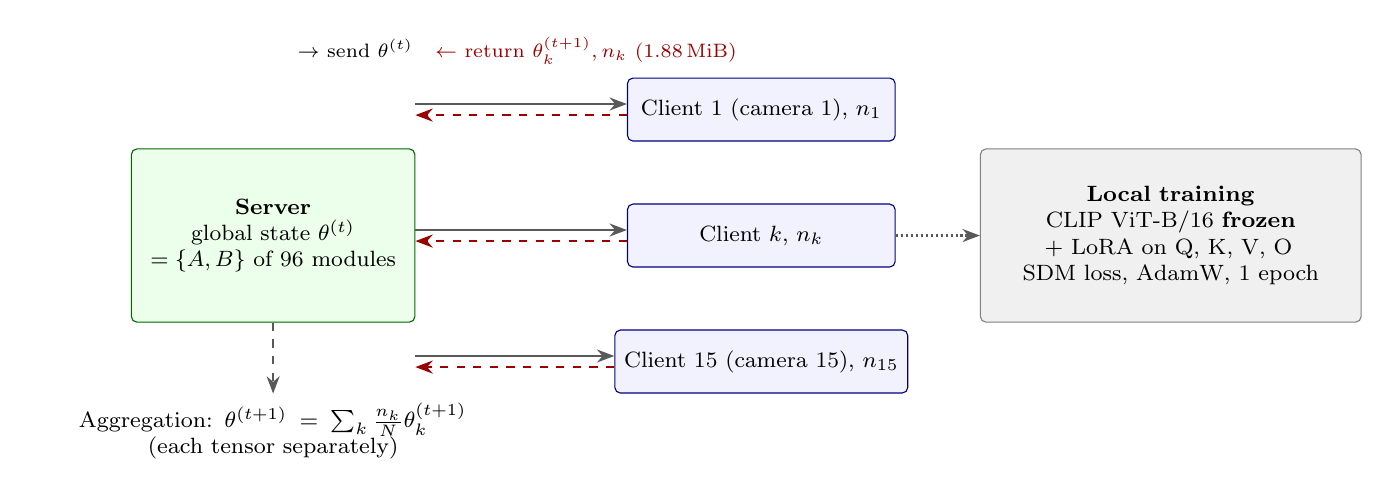
\begin{tikzpicture}[
  box/.style={draw,rounded corners=2pt,align=center,font=\footnotesize,minimum height=8mm,fill=blue!5,draw=blue!50!black},
  srv/.style={box,fill=green!8,draw=green!40!black,minimum width=36mm,minimum height=22mm},
  frz/.style={box,fill=black!6,draw=black!50,text width=46mm,minimum height=22mm},
  arr/.style={-{Stealth[length=2.2mm]},thick,draw=black!65}]
\node[srv] (S) at (0,0) {\textbf{Server}\\global state $\theta^{(t)}$\\$=\{A,B\}$ of 96 modules};
\node[box,minimum width=34mm] (c1) at (6.2,1.6) {Client 1 (camera 1), $n_1$};
\node[box,minimum width=34mm] (c2) at (6.2,0) {Client $k$, $n_k$};
\node[box,minimum width=34mm] (c3) at (6.2,-1.6) {Client 15 (camera 15), $n_{15}$};
\node[frz] (M) at (11.4,0) {\textbf{Local training}\\CLIP ViT-B/16 \textbf{frozen}\\+ LoRA on Q, K, V, O\\SDM loss, AdamW, 1 epoch};
\foreach \c in {c1,c2,c3}{
  \draw[arr] ([yshift=2pt]S.east |- \c.west) -- ([yshift=2pt]\c.west);
  \draw[arr,dashed,draw=red!60!black] ([yshift=-2pt]\c.west) -- ([yshift=-2pt]S.east |- \c.west);
}
\draw[arr,densely dotted] (c2.east) -- (M.west);
\node[font=\scriptsize] at (3.1,2.35) {$\rightarrow$ send $\theta^{(t)}$\quad\textcolor{red!60!black}{$\leftarrow$ return $\theta_k^{(t+1)},n_k$ (\numUplinkLoRA\,MiB)}};
\node[align=center,font=\footnotesize,below=9mm of S,text width=60mm] (agg) {Aggregation: $\theta^{(t+1)}=\sum_k\frac{n_k}{N}\theta_k^{(t+1)}$\\(each tensor separately)};
\draw[arr,dashed] (S) -- (agg);
\end{tikzpicture}}
\caption{One FedAvg round. The clients send only the LoRA matrices (\numTrainable{} parameters). All clients use the same frozen CLIP model.}
\label{fig:pipeline}
\end{figure}

\subsection{Model}
\begin{itemize}[leftmargin=1.5em]
  \item Base model: \texttt{openai/clip-vit-base-patch16} (HuggingFace).
  \item Image size: $384{\times}128$, the same as IRRA, UP-Person and DM-Adapter. The code interpolates the position embedding from a $14{\times}14$ grid to a $24{\times}8$ grid (192 patches).
  \item Text: CLIP BPE tokenizer, length 77.
  \item Training augmentation: horizontal flip, pad and random crop, random erasing ($p=0.5$).
  \item One sample is one image and one of its two captions. Thus, one image gives two samples in each epoch.
\end{itemize}

\subsection{LoRA}\label{sec:lora}
The code replaces each linear layer with the name \texttt{q\_proj}, \texttt{k\_proj}, \texttt{v\_proj} or \texttt{out\_proj} by $y=Wx+\frac{\alpha}{r}BAx$, with $r=4$ and $\alpha=8$. $W$ is frozen. $A$ has Kaiming initialization. $B$ starts at zero, so the model starts equal to CLIP. The code applies LoRA to both encoders: $12\text{ layers}\times4\text{ matrices}\times2\text{ encoders}=96$ modules. All other parameters are frozen.

The number of trainable parameters is: $48\times4\times(768+768)=294\,912$ (image encoder, width 768) plus $48\times4\times(512+512)=196\,608$ (text encoder, width 512). The total is \textbf{\numTrainable} of \numTotalParams{} parameters (\numTrainPct\%). This value agrees with \texttt{args.json}.

Difference from UP-Person: UP-Person puts LoRA only on K and V, with $r=16$ on RSTPReid, and adds a prefix and an adapter. Thus, we do not compare our numbers directly with UP-Person as ``PEFT against PEFT''.

\subsection{Loss}
The loss is SDM (\cref{eq:sdm}). Our code uses binary labels by identity. The IRRA code also gives a soft weight of 0.3 to ``same person, different image''. We did not measure the effect of this difference.

\subsection{FedAvg}
\Cref{alg:fedavg} shows one run. One GPU cannot hold 15 CLIP models. Thus, the code keeps one model and trains the clients one after the other. All clients start from the same global state, so the result is the same as parallel FedAvg.

\begin{algorithm}[t]
\caption{FedAvg with LoRA ($E=1$ local epoch, batch size 64)}\label{alg:fedavg}
\KwIn{clients $\mathcal{K}$ ($|\mathcal{K}|=15$), rounds $T$, learning rate $\eta_t$}
Set $\theta^{(1)}$: $A$ with Kaiming initialization, $B=0$, for the 96 modules\;
\For{$t=1,\dots,T$}{
  \ForEach{client $k\in\mathcal{K}$}{
    load $\theta^{(t)}$; make a new AdamW optimizer with learning rate $\eta_t$\;
    train $A,B$ for $E$ epochs on $\mathcal{D}_k$ with SDM; clip the gradient norm at 5\;
    send $\theta_k^{(t+1)}$ and $n_k=|\mathcal{D}_k|$ to the server\;
  }
  $\theta^{(t+1)}\gets\sum_k\frac{n_k}{N}\theta_k^{(t+1)}$, with $N=\sum_k n_k$ \tcp*{each tensor separately}
  each \texttt{eval\_every} rounds: test $\theta^{(t+1)}$ on the central test set\;
}
\end{algorithm}

Other settings from the code: AMP with fp16 (the loss is in fp32), \texttt{drop\_last=True}. The optimizer is new for each client in each round. This is correct for FedAvg, because the clients have no state.

\paragraph{Communication cost.} Each client sends \numTrainable{} fp32 values in each round: \numUplinkLoRA\,MiB. Full fine-tuning sends \numUplinkFull\,MiB. The ratio is \numUplinkRatio$\times$. For 15 clients, one round is \numUplinkRoundLoRA\,MiB (full fine-tuning: \numUplinkRoundFull\,GiB).

\paragraph{Inference.} The server deploys one global model: frozen CLIP + the averaged LoRA. The local LoRA states are only inputs to the average.

\subsection{Known limitation: LoRA aggregation bias}\label{sec:bias}
FedAvg averages $A$ and $B$ separately. With $s=\alpha/r$:
\begin{equation}\label{eq:bias}
s\Big(\sum_k\tfrac{n_k}{N}B_k\Big)\Big(\sum_k\tfrac{n_k}{N}A_k\Big)\;\neq\;s\sum_k\tfrac{n_k}{N}B_kA_k .
\end{equation}
This gives three problems:
\begin{enumerate}[label=(\alph*)]
  \item \textbf{Cross terms.} The product contains $B_kA_{k'}$ with $k\neq k'$. It mixes the factors of different clients.
  \item \textbf{Rank.} The correct average can have rank up to $Kr$. The averaged factors give rank $\le r$.
  \item \textbf{Non-unique factors.} $BA=(BT)(T^{-1}A)$ for each invertible $T$. Two clients can learn the same $\Delta W$ with different $A$ and $B$.
\end{enumerate}
The baseline accepts this bias. Known corrections are FFA-LoRA \citep{sun2024improvingloraprivacypreservingfederated} (freeze $A$, average only $B$), FLoRA \citep{wang2024florafederatedfinetuninglarge} and LoRA-FAIR \citep{bian2025lorafairfederatedlorafinetuning}. FedIT \citep{zhang2024buildingfederatedgptfederated} also identifies the problem. We did not run these methods yet.

\section{Experimental setup}\label{sec:setup}

\subsection{Data and camera partition}\label{sec:partition}
The RSTPReid training set has \numTotImg{} images, \numTotID{} identities and 37\,010 captions. Each file name contains the camera ID. Each camera is one client, so there are 15 clients. The server keeps the test set: 200 identities, 1\,000 gallery images and 2\,000 text queries. \Cref{tab:partition} in \cref{app:tables} gives the data of each client.

\result{The camera partition is not a uniform non-IID split. It has three properties:
(1)~the client sizes are very different;
(2)~the cameras make two groups that share almost no identities;
(3)~FedAvg gives the large clients a weight that is approximately proportional to $n_k^2$.}

\begin{enumerate}[leftmargin=1.5em]
  \item \textbf{Size.} A client has from \numImgMin{} to \numImgMax{} images (ratio \numImgRatio). The CV of the size is \numCVSize. The five largest clients have \numFiveShareNom\% of the data.
  \item \textbf{Two groups.} One identity is on 4.21 cameras on average. Only 0.2\% of the identities are on one camera only. But the containment matrix $|A\cap B|/\min(|A|,|B|)$ shows two blocks:
  \begin{itemize}
    \item \textbf{Group A}: cameras 1, 3, 5, 7, 14, 15 (\numImgA{} images, \numShareA\%).
    \item \textbf{Group B}: cameras 2, 6, 8, 9, 10, 11, 12, 13 (\numImgB{} images, \numShareB\%).
    \item \textbf{Bridge}: camera 4 (\numShareC\%).
  \end{itemize}
  Inside a group, the cameras share many identities (for example, 0.92 for cameras 1 and 7). Between the groups, they share almost none (0.02 for cameras 1 and 2). Thus, the skew is domain skew inside a group and label skew between the groups. The mean pairwise Jaccard (0.124, in \texttt{partition\_stats.json}) hides this structure.
  \item \textbf{Effective weight.} With $E=1$, client $k$ does $S_k=\lfloor n_k/64\rfloor$ steps. FedAvg multiplies the update by $n_k/N$. Thus, the effective weight is approximately proportional to $n_kS_k\propto n_k^2$ \citep{wang2020tacklingobjectiveinconsistencyproblem}. The two largest clients have \numTwoShareNom\% of the data, but \numTwoShareEff\% of the update. The smallest client has \numNomTwo\% of the data, but only \numEffTwo\% of the update. Also, \texttt{drop\_last=True} removes 42.9\% of the samples of the smallest client.
\end{enumerate}

\subsection{Runs}
All runs use: seed 42, CLIP ViT-B/16, image size $384{\times}128$, LoRA $r=4$, $\alpha=8$ on Q, K, V, O, batch size 64, AdamW (peak learning rate $10^{-4}$, weight decay 0.02), $\tau=0.02$, one local epoch, gradient clip 5.0, AMP. The test always uses the global model on the central test set. \Cref{tab:runs} gives the three runs.

\begin{table}[t]
\centering\small
\caption{The three runs (from \texttt{args.json} and \texttt{log.csv}). B5 run 1 and run 2 have the same settings. Only the planned number of rounds is different. With a constant learning rate, this number has no effect on the training.}\label{tab:runs}
\fit{\begin{tabular}{l l l l l l l}
\toprule
Run & Setting & Planned & Completed & Test & Learning rate & Optimizer\\
\midrule
C1-true & centralized (1 client) & 20 epochs & 20 & each epoch & cosine, 3 warm-up rounds & one AdamW for the full run\\
B5 run 1 & FL, 15 camera clients & 50 rounds & \numBoneLast{} (stopped) & each 5 rounds & constant $10^{-4}$ & new AdamW each round\\
B5 run 2 & FL, 15 camera clients & 25 rounds & \numBtwoLast{} (stopped) & each 5 rounds & constant $10^{-4}$ & new AdamW each round\\
\bottomrule
\end{tabular}}
\end{table}

\Cref{tab:grid} shows the full experiment plan. Only C1-true and B5 have results now. Thus, we cannot measure the non-IID gap and the PEFT gap yet.

\begin{table}[t]
\centering\small
\caption{Experiment plan (from \texttt{experiments/README.md}) and status.}\label{tab:grid}
\fit{\begin{tabular}{l l l l l}
\toprule
ID & Setting & Data split & Tuning & Status\\
\midrule
B2 & FL & IID & full & not run\\
B3 & FL & IID & LoRA & not run\\
B4 & FL & camera & full & not run\\
\textbf{B5} & FL & camera & LoRA $r=4$ & \textbf{2 runs, both stopped early}\\
C1 & centralized, new optimizer each epoch & -- & LoRA & not run\\
\textbf{C1-true} & centralized, one optimizer & -- & LoRA $r=4$ & \textbf{complete (20 epochs)}\\
Rank sweep & FL & camera & LoRA $r\in\{2,8,16\}$ & notebook cells exist, no results\\
\bottomrule
\end{tabular}}
\end{table}

\caution{Both B5 runs stopped early (possibly a Colab disconnect). C1-true uses a different learning-rate schedule and optimizer setting than B5. All runs use one seed only.}

\section{Results}\label{sec:results}

The script \texttt{scripts/gen\_tables.py} makes all numbers in this section from \texttt{results/*.csv}.

\subsection{Centralized LoRA (C1-true)}\label{sec:ceiling}

\result{With $r=4$ (\numTrainPct\% of the parameters) and SDM only, the centralized model converges at R@1 $=\numCPlatR\pm\numCPlatRsd$ and mAP $=\numCPlatM\pm\numCPlatMsd$ (mean of epochs 15--20). The peak R@1 (\numCBestR) is \numCOverR\pp{} higher than the converged value. Report the converged value and mAP, not the peak R@1.}

\Cref{fig:curves} shows the test curves. The training loss decreases from \numCFirstLoss{} to \numCFinalLoss{} and continues to decrease at epoch 20. The test metrics are flat after approximately epoch 8. Thus, the model is not limited by capacity. It starts to overfit.

\paragraph{R@1 is a noisy selection criterion.} In epochs 10--20, the coefficient of variation is \numCVR{} for R@1 and \numCVM{} for mAP. R@1 counts only the first position of 2\,000 queries, so its binomial standard error is approximately 1.1\pp. mAP uses the full ranking. The code saves \texttt{best.pt} at the highest R@1. Thus, it selects epoch \numCBestRround{} (R@1 \numCBestR, mAP \numCBestRmAP). The best mAP is at epoch \numCBestMround{} (\numCBestM). The model at epoch \numCBestRround{} is not better. It has a lucky top-1 result.

\begin{figure}[t]
\centering
\begin{tikzpicture}
\begin{groupplot}[group style={group size=2 by 1,horizontal sep=1.6cm},width=0.49\textwidth,height=5.6cm,
  xlabel={Round (FL) / epoch (centralized)},grid=major,grid style={dotted,gray!50},tick label style={font=\footnotesize},
  label style={font=\footnotesize},legend style={font=\scriptsize,at={(0.98,0.04)},anchor=south east,draw=none,fill=white,fill opacity=0.8}]
\nextgroupplot[ylabel={R@1 (\%)},ymin=40,ymax=62,xmin=0,xmax=35]
\addplot[black,thick,mark=*,mark size=1.2pt] table[col sep=comma,x=round,y=r1] {generated/curve_c1.csv};
\addplot[blue!70!black,thick,mark=square*,mark size=1.6pt] table[col sep=comma,x=round,y=r1] {generated/curve_b5v1.csv};
\addplot[red!70!black,thick,mark=triangle*,mark size=1.8pt] table[col sep=comma,x=round,y=r1] {generated/curve_b5v2.csv};
\addplot[gray,dashed,domain=0:35] {\numIrraConvR};
\legend{C1-true (centralized),B5 run 1 (FL),B5 run 2 (FL),IRRA converged}
\nextgroupplot[ylabel={mAP (\%)},ymin=30,ymax=48,xmin=0,xmax=35]
\addplot[black,thick,mark=*,mark size=1.2pt] table[col sep=comma,x=round,y=map] {generated/curve_c1.csv};
\addplot[blue!70!black,thick,mark=square*,mark size=1.6pt] table[col sep=comma,x=round,y=map] {generated/curve_b5v1.csv};
\addplot[red!70!black,thick,mark=triangle*,mark size=1.8pt] table[col sep=comma,x=round,y=map] {generated/curve_b5v2.csv};
\addplot[gray,dashed,domain=0:35] {\numIrraConvM};
\end{groupplot}
\end{tikzpicture}
\caption{Test curves on RSTPReid. Dashed line: IRRA converged value (mean of epochs 51--60 in the IRRA log). B5 has a test each 5 rounds. B5 run 1 stopped at round \numBoneLast{}, run 2 at round \numBtwoLast{}. One FL round has approximately the same number of optimizer steps as one centralized epoch.}
\label{fig:curves}
\end{figure}

\subsection{Comparison with IRRA (full fine-tuning)}\label{sec:vsirra}

\result{On the same converged measure, centralized LoRA + SDM is \numGapIrraConvR\pp{} R@1 and \numGapIrraConvM\pp{} mAP below IRRA. It is not approximately 3\pp{}. That value compares the IRRA peak (60.20) with our converged value. The gap contains two causes: PEFT, and the ID + MLM losses of IRRA. The current data cannot separate them.}

\begin{table}[t]
\centering\small
\caption{Comparison on the same measure. ``Peak'': maximum of all tests. ``Converged'': mean $\pm$ standard deviation of the last tests (IRRA: epochs 51--60; C1-true: epochs 15--20). $^{a}$Log in \texttt{data/irra\_rtsp} with \texttt{loss\_names: sdm+id+mlm}. Its timestamp is 2023-03-17, so it is probably the log that the IRRA authors released. We did not confirm the source. $^{b}$One seed. $^{c}$One test at round 30. The run stopped at round \numBoneLast.}\label{tab:vsirra}
\fit{\begin{tabular}{l r l cc cc}
\toprule
 & & & \multicolumn{2}{c}{Peak (best of $N$)} & \multicolumn{2}{c}{Converged (mean)}\\
\cmidrule(lr){4-5}\cmidrule(lr){6-7}
Setting & Params & Loss & R@1 & mAP & R@1 & mAP\\
\midrule
IRRA, full FT$^{a}$ & 195M & SDM+ID+MLM & 60.20 & 47.17 & 58.73\,$\pm$\,0.22 & 46.65\,$\pm$\,0.03\\
C1-true: LoRA $r{=}4$, centralized$^{b}$ & 0.49M & SDM & 58.85 & 45.56 & 57.18\,$\pm$\,0.28 & 45.42\,$\pm$\,0.13\\
B5 (run 1): LoRA $r{=}4$, FL camera$^{c}$ & 0.49M & SDM & -- & -- & 57.05 (r.30) & 44.63 (r.30)\\
\bottomrule
\end{tabular}
}
\end{table}

Notes on \cref{tab:vsirra}:
\begin{itemize}[leftmargin=1.5em]
  \item The IRRA value 60.20 is the peak at epoch \numIrraBestEp{} of \numIrraNEval{} tests. The converged value is \numIrraConvR.
  \item UP-Person reports 63.15 R@1 on RSTPReid. Our pipeline is $\ge4.3$\pp{} below. UP-Person uses LoRA on K and V with $r=16$, plus a prefix and an adapter (\cref{sec:lora}). We do not know if its value is a peak or a converged value.
  \item The IRRA README has a ``CLIP baseline'' row with 54.05 R@1. We did not confirm the loss settings of this row. Thus, we do not use it for conclusions.
\end{itemize}

\subsection{FL compared with centralized training}\label{sec:flgap}

\result{At the same round, the gap between FL and centralized training decreases in mAP: from more than 6\pp{} at round 5 to less than 1\pp{} at round 30. The FL model continues to improve when it stops. The data agree with the hypothesis ``FL needs more rounds, but it does not lower the final accuracy''. The data do not prove it, because the FL runs did not reach a flat curve.}

\Cref{tab:flgap} compares B5 with C1-true at the same round. One FL round has 571 steps in total on the 15 clients. One centralized epoch has 578 steps. Thus, the comparison uses the same compute. In mAP, $\Delta$ decreases at each test in both runs. In R@1, the trend is the same, but with more noise.

\begin{table}[t]
\centering\small
\caption{Gap between centralized and FL training at the same round. $\Delta_i=\text{C1-true}-\text{B5 run }i$ (percentage points). $^\dagger$C1-true is flat, so the value is the converged value (mean of epochs 15--20). ``--'': run 2 stopped at round \numBtwoLast. C1-true and B5 use different learning-rate and optimizer settings. Thus, $\Delta$ is an indication, not a clean measurement.}\label{tab:flgap}
\fit{\begin{tabular}{r cc c}
\toprule
Round & Centralized & Federated & $\Delta$\\
\midrule
\multicolumn{4}{l}{\textit{R@1 (\%)}}\\
5 & 54.15 & 46.95 & 7.20\\
10 & 57.00 & 52.55 & 4.45\\
15 & 57.55 & 54.15 & 3.40\\
20 & 56.95 & 56.00 & 0.95\\
25 & 57.18$^\dagger$ & 57.05 & 0.13\\
30 & 57.18$^\dagger$ & 57.05 & 0.13\\
\midrule
\multicolumn{4}{l}{\textit{mAP (\%)}}\\
5 & 42.64 & 36.60 & 6.04\\
10 & 45.19 & 40.26 & 4.92\\
15 & 45.35 & 42.05 & 3.30\\
20 & 45.42 & 43.34 & 2.08\\
25 & 45.42$^\dagger$ & 44.23 & 1.19\\
30 & 45.42$^\dagger$ & 44.63 & 0.79\\
\bottomrule
\end{tabular}
}
\end{table}

\paragraph{Noise between two equal runs.} B5 run 1 and run 2 have the same settings. Thus, their difference is an estimate of the run-to-run noise (\cref{tab:noise}). The maximum difference is \numNoiseR\pp{} in R@1 and \numNoiseM\pp{} in mAP. A difference in R@1 that is less than approximately 1.7\pp{} is not different from noise. This includes $\Delta$ at round 20. The mAP gap at round 30 is only approximately two times the mAP noise. We must use more seeds in the next runs.

\begin{table}[t]
\centering\small
\caption{Two B5 runs with the same settings. The difference is a rough estimate of the run-to-run noise (two values at each round only).}\label{tab:noise}
\begin{tabular}{r cc cc}
\toprule
 & \multicolumn{2}{c}{R@1} & \multicolumn{2}{c}{mAP}\\
\cmidrule(lr){2-3}\cmidrule(lr){4-5}
Round & run 1 & run 2 & run 1 & run 2\\
\midrule
5 & 46.95 & 47.50 & 36.60 & 36.51\\
10 & 52.55 & 53.55 & 40.26 & 40.64\\
15 & 54.15 & 55.85 & 42.05 & 42.33\\
20 & 56.00 & 56.20 & 43.34 & 43.30\\
\bottomrule
\end{tabular}

\end{table}

\paragraph{Communication.} One round with 15 clients sends \numUplinkRoundLoRA\,MiB. After 30 rounds, the log shows \numUplinkRthirty\,MiB in total. Full fine-tuning needs approximately \numUplinkFullThirty\,GiB for 30 rounds (estimate from the parameter count).

\subsection{Differences between clients in FL}\label{sec:hetero}

\result{The mean training loss decreases at each round. But the clients do not converge at the same rate. The loss separates into two bands that agree with the two identity groups (\cref{sec:partition}). The gap between the groups increases from \numGapFirst{} to \numGapLast. This is a result on the training loss only. We did not show that the retrieval accuracy for group B is lower.}

The data come from \texttt{client\_loss.csv} of B5 run 2 (\numLastRound{} rounds $\times$ 15 clients). \Cref{tab:group} and \cref{fig:group} give the results:
\begin{itemize}[leftmargin=1.5em]
  \item The CV of the loss between the 15 clients increases from \numCVFirst{} (round 1) to \numCVLast{} (round \numLastRound).
  \item The gap between group B and group A increases from \numGapFirst{} to \numGapLast.
  \item The two trends are not monotonic. In \numSteps{} steps from one round to the next, the gap decreases \numGapDown{} times and the CV decreases \numCVDown{} times.
  \item Client \numLowClient{} (the largest camera) has the lowest loss in \numLowCount{} of \numLastRound{} rounds. Client \numHiOne{} has the highest loss in \numHiOneCount{} rounds.
  \item The correlation between client size and final loss is $r=\numPearsonAll$ ($r=\numPearsonNoTwo$ without client 2, which does only 1 step in each round). \Cref{tab:clientloss} in \cref{app:tables} gives all clients.
\end{itemize}

\begin{table}[t]
\centering\small
\caption{Mean SDM training loss of each camera group, B5 run 2. The CV uses the 15 clients (population standard deviation / mean).}\label{tab:group}
\begin{tabular}{r ccc c c}
\toprule
Round & Group A & Group B & Bridge (c4) & Gap $B{-}A$ & CV across clients\\
\midrule
1 & 24.25 & 26.84 & 27.32 & 2.58 & 0.072\\
5 & 16.73 & 20.17 & 20.89 & 3.44 & 0.131\\
10 & 14.81 & 18.76 & 19.67 & 3.96 & 0.163\\
15 & 13.90 & 18.13 & 18.83 & 4.23 & 0.179\\
21 & 12.79 & 17.34 & 17.86 & 4.55 & 0.200\\
\bottomrule
\end{tabular}

\end{table}

\begin{figure}[t]
\centering
\begin{tikzpicture}
\begin{groupplot}[group style={group size=2 by 1,horizontal sep=1.6cm},width=0.49\textwidth,height=5.4cm,
  xlabel={Round},grid=major,grid style={dotted,gray!50},tick label style={font=\footnotesize},label style={font=\footnotesize},
  legend style={font=\scriptsize,draw=none,fill=white,fill opacity=0.8}]
\nextgroupplot[ylabel={Mean SDM loss of the group},xmin=1,xmax=21,legend pos=north east]
\addplot[blue!70!black,thick,mark=*,mark size=1.2pt] table[col sep=comma,x=round,y=groupA] {generated/group_loss.csv};
\addplot[red!70!black,thick,mark=square*,mark size=1.4pt] table[col sep=comma,x=round,y=groupB] {generated/group_loss.csv};
\addplot[green!40!black,thick,dashed] table[col sep=comma,x=round,y=bridge] {generated/group_loss.csv};
\legend{Group A,Group B,Bridge (c4)}
\nextgroupplot[ylabel={CV of the loss between clients},xmin=1,xmax=21]
\addplot[black,thick,mark=*,mark size=1.2pt] table[col sep=comma,x=round,y=cv] {generated/group_loss.csv};
\end{groupplot}
\end{tikzpicture}
\caption{Left: mean training loss of each group. Right: spread of the loss between the 15 clients.}
\label{fig:group}
\end{figure}

\paragraph{Possible causes (hypotheses).}
\begin{enumerate}[leftmargin=1.5em]
  \item \textbf{Effective weight $\propto n_k^2$} (\cref{sec:partition}). Group A has the four largest clients (14, 1, 5, 7). Thus, the global update moves toward the minimum of group A.
  \item \textbf{LoRA rank limit} (\cref{sec:bias}). The two groups are almost two domains. They possibly need two different adaptation directions. The averaged factors give rank $\le4$ only. A rank sweep can test this hypothesis: if a higher $r$ decreases the gap, hypothesis 2 is correct. If the gap does not change, cause 1 is more probable.
\end{enumerate}

\caution{Two items make the conclusion ``FedAvg leaves group B behind'' weaker.
(1)~The values are training losses on the data of each client. \texttt{evaluate.py} does not know which test identity is in which group.
(2)~The gap is already \numGapFirst{} at round 1. Thus, part of the gap can come from the data of group B (for example, camera 10 has 1.80 images per identity, most cameras have approximately 1.0), and not from FedAvg.
To test this, (a)~label the 200 test identities as A, B or bridge and calculate R@1 and mAP for each group, and (b)~calculate the loss of the centralized model on the data of each group.}

\section{Limitations and open items}\label{sec:limits}

\Cref{tab:claims} gives the status of each claim. ``Needs evidence'' is a task list. Do not use these claims in the thesis before the related task is complete.

\begin{table}[t]
\centering\small
\caption{Claims and evidence. ``Published'': value from the authors, not reproduced. ``Run'': value from \texttt{results/}.}\label{tab:claims}
\begin{tabularx}{\textwidth}{>{\raggedright\arraybackslash}p{6.2cm} >{\raggedright\arraybackslash}p{3.2cm} X}
\toprule
Claim & Evidence & Status\\
\midrule
PEFT is equal to or better than full fine-tuning in TBPS & \Cref{tab:ftvspeft} (published) & Supported by published values\\
SDM alone is sufficient for PEFT & UP-Person ablation (published) & Supported in centralized PEFT; not tested in our pipeline\\
LoRA $r=4$ sends \numUplinkLoRA\,MiB per client per round & \texttt{args.json} (run) & Supported\\
Centralized LoRA converges at R@1 \numCPlatR, mAP \numCPlatM & C1-true (run) & Supported, one seed\\
Gap to IRRA is approx.\ \numGapIrraConvR\pp{} R@1 (converged) & \Cref{tab:vsirra} & Supported; mixes PEFT and loss effects\\
FL needs more rounds, but it does not lower the final accuracy & \Cref{tab:flgap} & \textbf{Needs evidence}: FL did not reach a flat curve; R@1 noise approx.\ 1.7\pp\\
The client loss separates into two groups & \Cref{tab:group} & Supported (training loss, not monotonic)\\
FedAvg gives lower retrieval accuracy for group B & -- & \textbf{Needs evidence}: test by group\\
LoRA rank limit causes the group gap & -- & \textbf{Needs evidence}: rank sweep\\
PEFT gap and non-IID gap & -- & \textbf{Not measured}: B3, B4 not run\\
First work that combines FL, PEFT, CLIP and TBPS & Literature study & \textbf{Needs evidence}: systematic survey\\
\bottomrule
\end{tabularx}
\end{table}

Other limitations:
\begin{itemize}[leftmargin=1.5em]
  \item One dataset (RSTPReid) and one partition (camera). The results can be different on other data.
  \item The report does not measure privacy. FL alone does not guarantee privacy.
  \item Our SDM does not use the soft weight for ``same person, different image'' that IRRA uses.
\end{itemize}

\section{Next steps}\label{sec:next}

The order of the tasks is: first make the current measurements reliable, then add new methods.

\begin{table}[t]
\centering\small
\caption{Next tasks, in order of priority.}\label{tab:next}
\begin{tabularx}{\textwidth}{c >{\raggedright\arraybackslash}p{6.4cm} X}
\toprule
\# & Task & Purpose\\
\midrule
\multicolumn{3}{l}{\textit{Group 1 -- make the baseline reliable}}\\
1 & Run B5 again with the C1-true settings (cosine schedule), until the curve is flat, with $\ge3$ seeds & Measure the FL gap correctly\\
2 & Run C1 (centralized, new optimizer each epoch) & Separate the effect of the data split from the effect of the optimizer reset\\
3 & Label the test identities by group; calculate R@1 and mAP for each group & Test ``FedAvg leaves group B behind''\\
4 & Save \texttt{best.pt} at the highest mAP, not R@1 & Do not select a noise peak\\
\multicolumn{3}{l}{\textit{Group 2 -- complete the experiment plan}}\\
5 & B3 (IID, LoRA) & Measure the non-IID gap\\
6 & B4 (camera, full) and centralized full fine-tuning with SDM only & Measure the PEFT gap, separately from the loss effect\\
7 & Rank sweep $r\in\{2,4,8,16\}$ with $\alpha=2r$ & Test the rank-limit hypothesis\\
\multicolumn{3}{l}{\textit{Group 3 -- methods (possible contributions)}}\\
8 & FFA-LoRA, FLoRA, LoRA-FAIR in the same pipeline & Correct the aggregation bias (O2)\\
9 & FedNova normalization in \texttt{fedavg} & Correct the $n_k^2$ effective weight\\
10 & Clustered FL (IFCA \citep{ghosh2021efficientframeworkclusteredfederated}, CFL \citep{sattler2019clusteredfederatedlearningmodelagnostic}) for the two groups & Use the two-group structure\\
11 & UP-Person and DM-Adapter in FL & Test other PEFT methods under O2 and O3\\
\bottomrule
\end{tabularx}
\end{table}

Two tasks without experiments are also necessary: a systematic survey of FL + PEFT + vision-language models, and a reproduction of one UP-Person or DM-Adapter result with the code in \texttt{reference/}.

\section{Conclusion}\label{sec:conclusion}
We built a FedAvg + LoRA + CLIP + SDM pipeline for TBPS and trained it on RSTPReid with 15 camera clients. LoRA $r=4$ trains \numTrainPct\% of the parameters and sends \numUplinkLoRA\,MiB per client per round. The centralized LoRA model converges at R@1 \numCPlatR{} and mAP \numCPlatM. This is \numGapIrraConvR\pp{} R@1 below IRRA on the same measure. The FL model gets near this value when the number of rounds increases. The camera partition has two identity groups, and the training loss of the two groups separates during FL. The next tasks make these measurements reliable (more seeds, complete runs), then test methods for the LoRA aggregation bias and for the two-group non-IID data.


\bibliographystyle{unsrtnat}
\bibliography{refs}

\appendix
\section{Additional tables}\label{app:tables}

\begin{table}[H]
\centering\small
\caption{The 15 camera clients, in order of size. ``Steps/round'' $=\lfloor n_k/64\rfloor$, with $n_k$ the number of samples (captions). ``\% effective'' $\propto n_k\lfloor n_k/64\rfloor$ is the real part of the global update when $E=1$. Generated from \texttt{partition\_stats.json}.}\label{tab:partition}
\fit{\begin{tabular}{r c r r c r r r}
\toprule
Client (camera) & Group & Images & \% total & IDs & Img/ID & Steps/round & \% effective\\
\midrule
14 & A & 3\,265 & 17.6 & 2\,307 & 1.42 & 102 & 27.277\\
1 & A & 3\,071 & 16.6 & 2\,421 & 1.27 & 95 & 23.896\\
5 & A & 2\,504 & 13.5 & 2\,208 & 1.13 & 78 & 15.997\\
7 & A & 2\,045 & 11.1 & 1\,968 & 1.04 & 63 & 10.552\\
11 & B & 1\,820 & 9.8 & 1\,393 & 1.31 & 56 & 8.348\\
13 & B & 1\,521 & 8.2 & 1\,360 & 1.12 & 47 & 5.855\\
12 & B & 1\,187 & 6.4 & 1\,105 & 1.07 & 37 & 3.597\\
15 & A & 999 & 5.4 & 952 & 1.05 & 31 & 2.537\\
4 & bridge & 514 & 2.8 & 503 & 1.02 & 16 & 0.674\\
10 & B & 410 & 2.2 & 228 & 1.80 & 12 & 0.403\\
6 & B & 388 & 2.1 & 370 & 1.05 & 12 & 0.381\\
3 & A & 313 & 1.7 & 307 & 1.02 & 9 & 0.231\\
8 & B & 297 & 1.6 & 290 & 1.02 & 9 & 0.219\\
9 & B & 115 & 0.6 & 114 & 1.01 & 3 & 0.028\\
2 & B & 56 & 0.3 & 53 & 1.06 & 1 & 0.005\\
\bottomrule
\end{tabular}
}
\end{table}

\begin{table}[H]
\centering\small
\caption{SDM training loss of each client at the first and the last round, B5 run 2, in order of size. For clients with $\le12$ steps per round, the loss is a noisy estimate.}\label{tab:clientloss}
\fit{\begin{tabular}{r r r c c c c}
\toprule
Client & Samples & Steps/round & Group & Loss r.1 & Loss r.21 & Drop (\%)\\
\midrule
14 & 6\,530 & 102 & A & 21.18 & 10.49 & 50.5\\
1 & 6\,142 & 95 & A & 23.40 & 12.44 & 46.8\\
5 & 5\,008 & 78 & A & 23.83 & 12.94 & 45.7\\
7 & 4\,090 & 63 & A & 23.72 & 11.07 & 53.3\\
11 & 3\,640 & 56 & B & 26.34 & 17.62 & 33.1\\
13 & 3\,042 & 47 & B & 27.18 & 20.00 & 26.4\\
12 & 2\,374 & 37 & B & 26.22 & 16.17 & 38.4\\
15 & 1\,998 & 31 & A & 26.34 & 14.68 & 44.3\\
4 & 1\,028 & 16 & bridge & 27.32 & 17.86 & 34.6\\
10 & 820 & 12 & B & 27.51 & 20.27 & 26.3\\
6 & 776 & 12 & B & 26.54 & 14.72 & 44.5\\
3 & 626 & 9 & A & 27.06 & 15.10 & 44.2\\
8 & 594 & 9 & B & 27.56 & 19.16 & 30.5\\
9 & 230 & 3 & B & 27.57 & 18.15 & 34.2\\
2 & 112 & 1 & B & 25.77 & 12.60 & 51.1\\
\bottomrule
\end{tabular}
}
\end{table}

\begin{table}[H]
\centering\small
\caption{Estimated uplink per client per round (fp32, 4 bytes for each parameter) if a method sends all its trainable parameters. The first five parameter counts are published values. The last row is measured.}\label{tab:uplink}
\fit{\begin{tabular}{l l r r}
\toprule
Method & Tuning & Trainable params & Est. uplink (MiB/client/round)\\
\midrule
CFine & full & 205M & 782\\
IRRA & full & 195M & 744\\
CSKT & PETL & 12M & 46\\
DM-Adapter & PETL (MoE-Adapter) & 16M & 61\\
UP-Person & PETL (LoRA+Prefix+Adapter) & 7.4M & 28\\
\textbf{This pipeline} (LoRA $r{=}4$, Q,K,V,O) & LoRA & 0.49M & 1.88\\
\bottomrule
\end{tabular}
}
\end{table}

\section{How to reproduce}\label{app:repro}
\sloppy
\paragraph{Build the report.} In \texttt{paper/}, run \texttt{python3 scripts/gen\_tables.py}, then \texttt{latexmk -pdf -outdir=build main.tex}. On Overleaf, use pdfLaTeX. The folder \texttt{generated/} is in the repository, so Overleaf does not need Python. Run \texttt{gen\_tables.py} again after a change in \texttt{results/}.

\paragraph{Data sources.}
\begin{itemize}[leftmargin=1.5em]
  \item \texttt{results/B5\_v1\_log.csv}, \texttt{B5\_v2\_log.csv}, \texttt{B5\_v2\_client\_loss.csv}, \texttt{C1true\_log.csv}: copies from \texttt{data/runs/}.
  \item \texttt{results/partition\_stats.json}: copy from \texttt{data/rstpreid\_fl\_camera/}.
  \item \texttt{results/irra\_rstp\_train\_log.txt}, \texttt{irra\_rstp\_configs.yaml}: copies from \texttt{data/irra\_rtsp/}.
  \item Published values (\cref{tab:ftvspeft}) come from \texttt{docs/benchmark-baseline.md}.
\end{itemize}

\paragraph{Run commands.} See \texttt{experiments/README.md}. B5: \texttt{--partition camera --tuning lora --lora\_rank 4 --lora\_alpha 8}. C1-true: \texttt{--partition centralized --persistent\_optimizer --lr\_schedule cosine --warmup\_rounds 3 --eval\_every 1}.

\end{document}
